\begin{figure*}[t]
%\vspace{-0.1in}
\centering
\subfigure[Topology and flows] {
    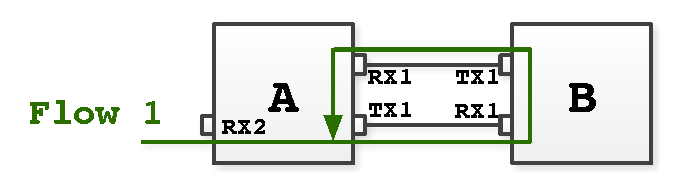
\includegraphics[width=0.33\textwidth] {figs/loop_case_topo_and_flow}
}
\subfigure[Buffer dependency graph]{
    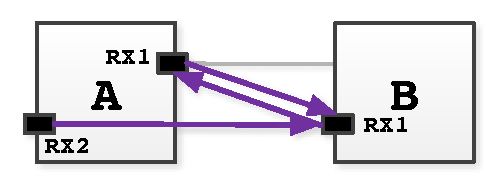
\includegraphics[width=0.25\textwidth] {figs/loop_case_ingress_buffer_dependency}
}
\subfigure[Stable state model]{
    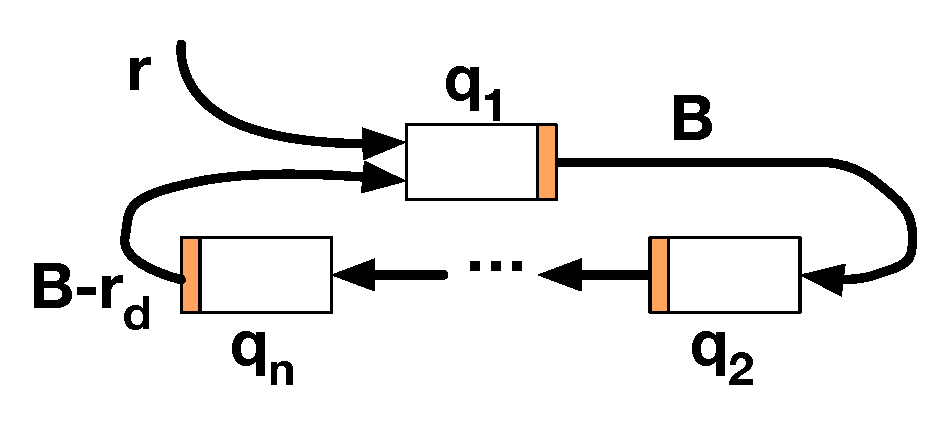
\includegraphics[width=0.25\textwidth] {figs/loop_analysis}
}
\vspace{-0.15in}
\caption{Single looping flow creates CBD but may not create deadlock.}
\vspace{-0.15in}
\label{fig:loop}
\end{figure*}

\secspacelarge
\section{Case Studies: CBD is Insufficient for Deadlock}
\label{sec:analysis}
\secspace

Although CBD is a necessary condition for deadlock, it is not a
sufficient condition. In this section, we present our case studies in which CBD
is present, but deadlock formation still depends on other factors. We demonstrate
that 1) a looping flow that generates CBD does not always lead to deadlock.
The length of loop, flow rates and packet Time-To-Live (TTL) affects whether
the deadlock forms. 2) Multiple flows may cause CBD,
but slightly different flow sets lead to different deadlock results. 3) Rate-limiting can
prevent deadlock from happening.

\secspace
\subsection{Case 1: Flow Rate and TTL Determine Deadlock in a Routing Loop}
\secspace

%A routing loop can create cyclic buffer dependency if a flow is trapped in the loop.
%The simplest example is a two-hop loop between two switches, as shown in Figure~\ref{fig:loop}(a).
%We then plot buffer dependency graph (Figure~\ref{fig:loop}(b)), $RX$ represents input
%queue (or port). Each directed line represents a buffer dependency from the source TX to the
%destination TX. For example, packets buffered in $RX1$ of switch A will be sent to either $RX1$
%of B, and vice versa. So in Figure~\ref{fig:loop}(b), two directed lines are drawn between A and B.
%Switch A's dependency on switch B means whether switch A can move
%the packets in its receiving buffer {\em RX1} to egress depends on switch B's buffer {\em RX1}.\footnote{We
%focus on receiving buffer because PFC PAUSE triggers based on the occupancy of receiving buffer.}
%The switches can send packets to the other side only
%when the other side's buffer utilization is under PFC PAUSE threshold. The deadlock happens when
%both of the involved buffers reach the PFC threshold at the same time and PAUSE the links.

A routing loop can create CBD if a flow is trapped in the loop.
\revise{The simplest example is a two-hop loop between two switches, as shown in Figure~\ref{fig:loop}(a) ($RX$ represents input
queue (or port), and $TX$ represents output queue (or port)). We then plot buffer dependency graph (Figure~\ref{fig:loop}(b)). Each directed line represents a buffer dependency from the source RX to the destination RX. For example, packets buffered in $RX1$ of switch A will be sent to $RX1$
of B, and vice versa.} So in Figure~\ref{fig:loop}(b), two directed lines are drawn between A and B.
Switch A's dependency on switch B means whether switch A can move
the packets in its receiving buffer {\em RX1} to egress depends on switch B's buffer {\em RX1}.\footnote{We
focus on receiving buffer because PFC PAUSE triggers based on the occupancy of receiving buffer.}
The switches can send packets to the other side only
when the other side's buffer utilization is under PFC PAUSE threshold. The deadlock happens when
both of the involved buffers reach the PFC threshold at the same time and PAUSE the links.


However, this CBD may not always turn into deadlock state. The flow
 rate, the TTL (time-to-live) of packets and the length of the loop together
determine whether there will be deadlock. In our testbed, we run a simple experiment on
two switches that are connected by a 40Gbps link and configured with a routing loop.
All packets have initial TTL of 16 and are injected into one of the switches. We find that,
only if the packet injection rate exceeds 5Gbps, there can form deadlock.

In order to analyze deadlock formation in the cases of routing loop, we develop a mechanism called
{\em boundary state analysis}. It yields accurate prediction of whether deadlock forms,
as shown below.

\para{Boundary state analysis.}
On any of the switches in the loop, packets are injected by the previous hop and drained by the next hop.
If the draining rate is smaller than the injecting rate, packets will continuously queue up in the
switch buffers. In a loop, once one switch buffers enough packets and triggers PFC, the PFC will soon
cascade through the whole loop and forms deadlock.
We define {\em boundary state}, in which the injecting rate and draining rate are balanced on every
switch, and any larger injecting rate leads to deadlock because draining rate cannot catch up.

We build the boundary state model as illustrated in
Figure~\ref{fig:loop}(c). The variables are described in Table~\ref{tab:stable_state}.


\begin{table}[h]
\centering
\vspace{-0.1in}
\caption{\small Stable state analysis variables}
\vspace{-0.15in}
\label{tab:stable_state}
{\small
\begin{tabular}{|c|c|}
 \hline
Variable &  Description \\
\hline
$r$ & Inject rate of new packets. \\
\hline
$B$ & Link bandwidth. \\
\hline
$r_d$ & Packets drain rate caused by TTL expiration. \\
\hline
$TTL$ & Initial Time-To-Live value. \\
\hline
$n$ & The length of the routing loop. \\
\hline
\end{tabular}
}
\vspace{-0.15in}
\end{table}

According to the boundary state definition, the injecting rate and draining rate
must be equal on the first switch:
\begin{equation}
\small
r + B - r_d = B
\label{eq:rate}
\end{equation}
In addition, we consider the sum of TTL values of all packets in the system.
During the boundary state, it should remain stable. Therefore, the increase
rate and decrease rate of the sum of TTL should be the same:
\begin{equation}
\small
n * B = TTL * r
\label{eq:ttl}
\end{equation}
Combining Equation~\ref{eq:rate}, Equation~\ref{eq:ttl}, and the fact that
deadlock requires larger injecting rate than that in boundary state, we derive the
{\em necessary and sufficient condition} of deadlock in a routing loop scenario:
\begin{equation}
\small
r > r_d = \frac{nB}{TTL}
\label{eq:condition}
\end{equation}
This matches what we observe in testbed experiment: with $B=40Gbps$, $n=2$ and
$TTL=16$, the flow injecting rate must be at least $5Gbps$ to cause deadlock. With larger bandwidth,
shorter loop length or smaller initial TTL values, the threshold of $r$ can be higher.
As long as the flow rate is smaller than the threshold, no deadlock will form.
As shown in Section~\ref{sec:mitigation}, we may utilize this property to avoid deadlock,
even if routing loop occurs.

\secspace
\subsection{Case 2: Traffic Matrix Affects Deadlock}
\secspace


\begin{figure*}[t]
	%\vspace{-0.1in}
	\centering
	\subfigure[Topology and flows] {
		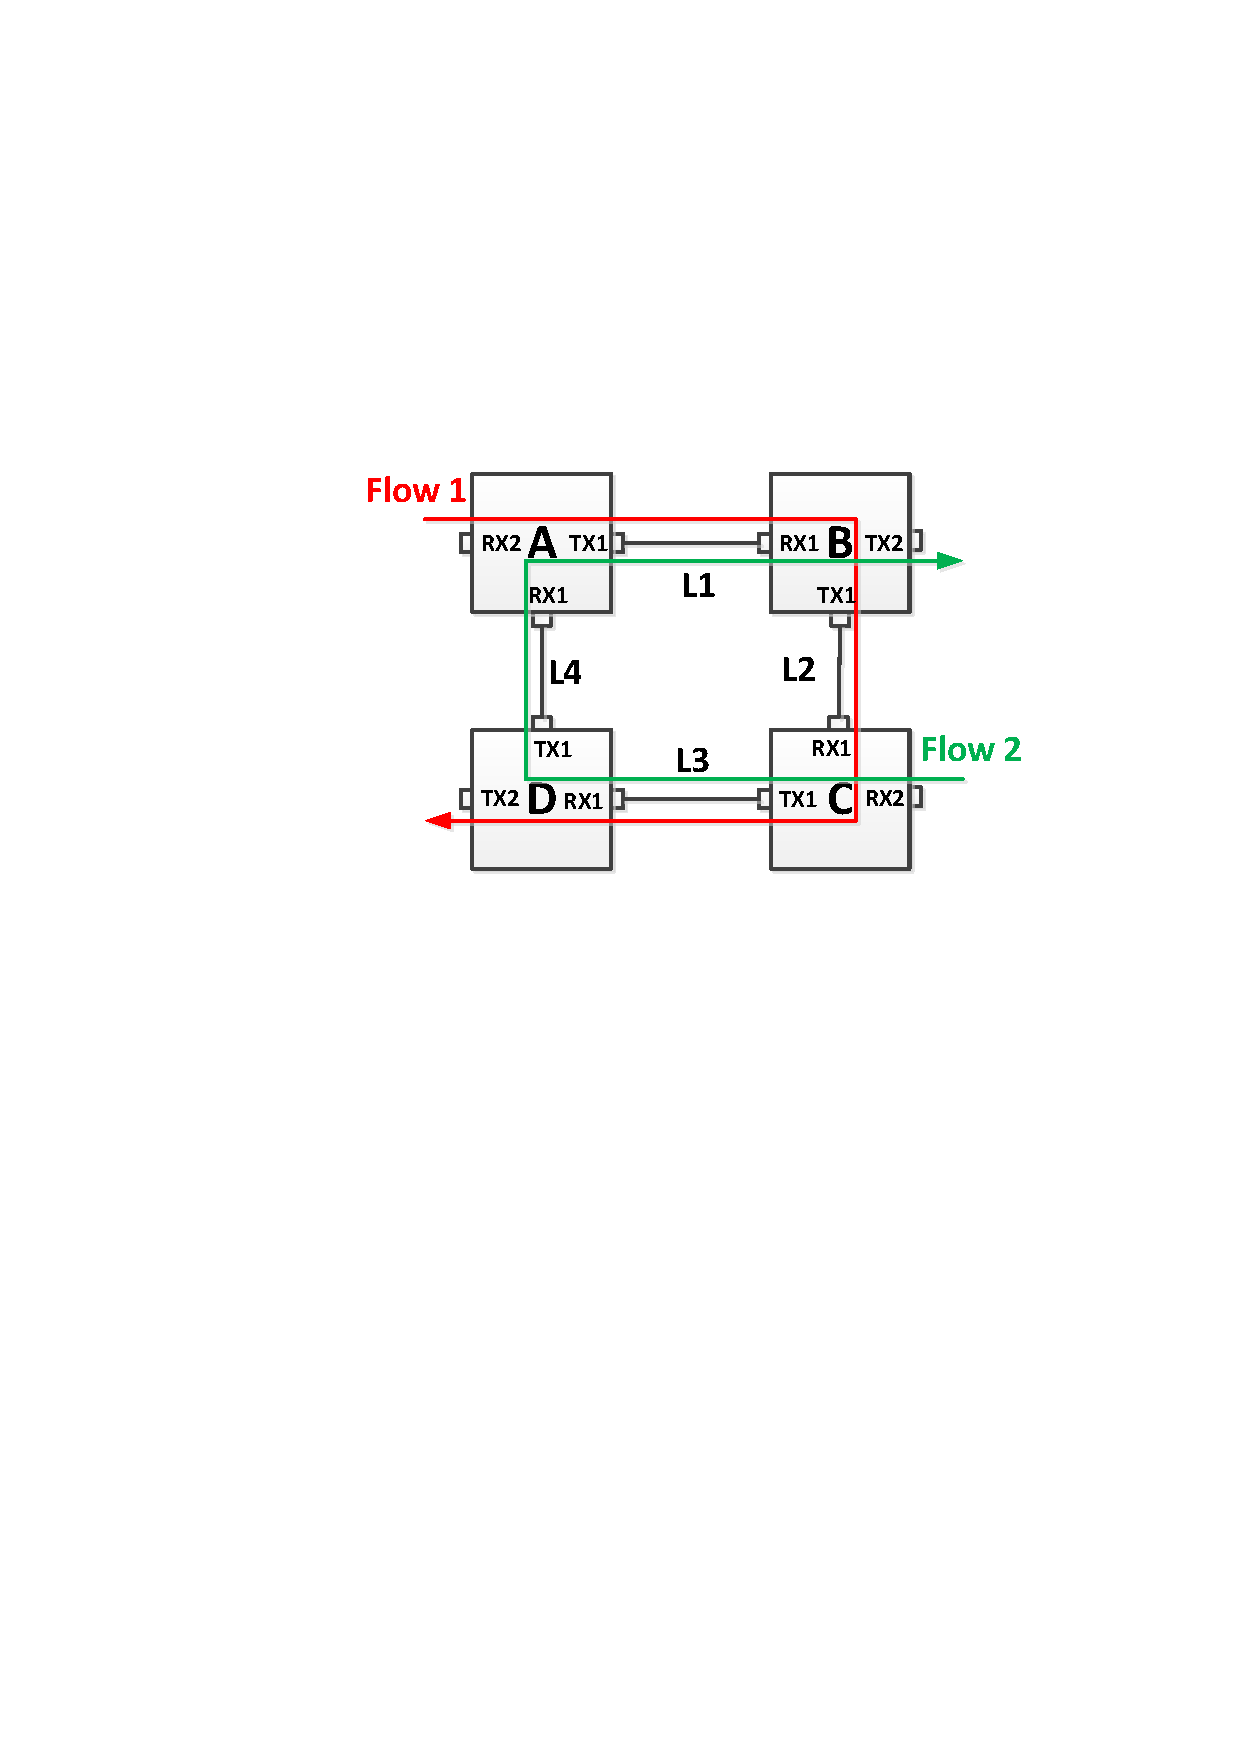
\includegraphics[width=0.28\textwidth] {figs/case1_topo.pdf}
	}
	\subfigure[Buffer dependency graph]{
		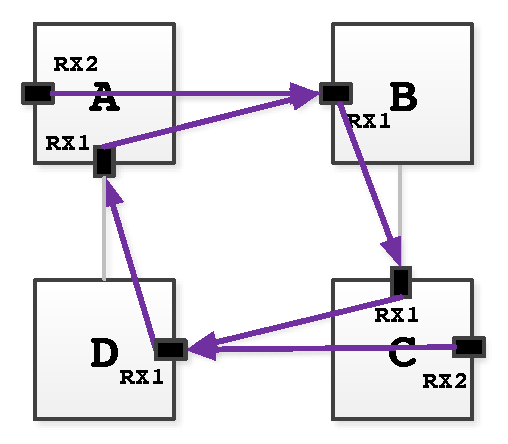
\includegraphics[width=0.19\textwidth] {figs/case1_buffer_dependency.pdf}
	}
	\subfigure[Pause events at four links]{
		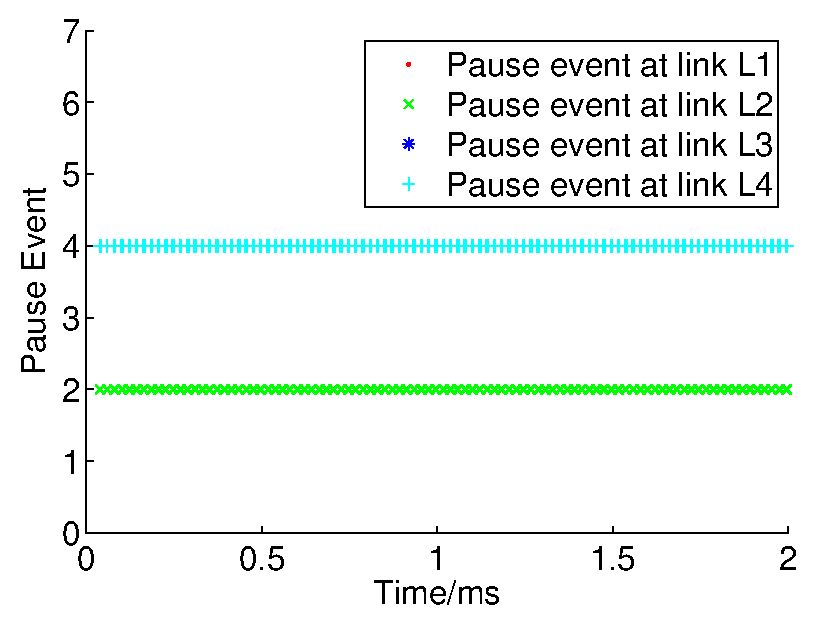
\includegraphics[width=0.2\textwidth] {figs/case1_pause.eps}
	}
	\vspace{-0.1in}
	
	\subfigure[Buffer occupancy at switch A] {
		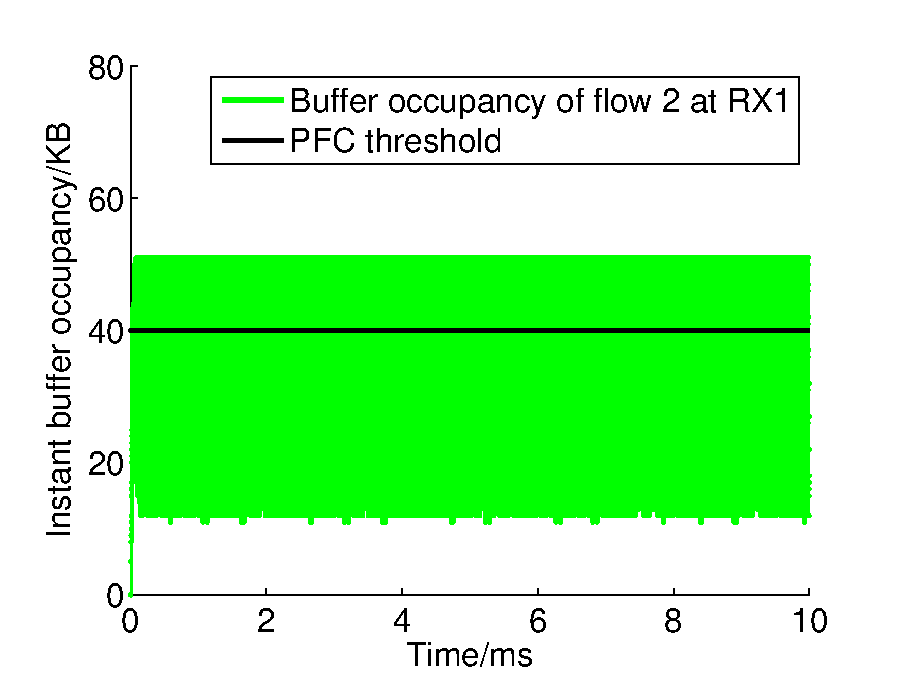
\includegraphics[width=0.23\textwidth] {figs/case1_buffer_occupancy_A.eps}
	}
	\subfigure[Buffer occupancy at switch B] {
		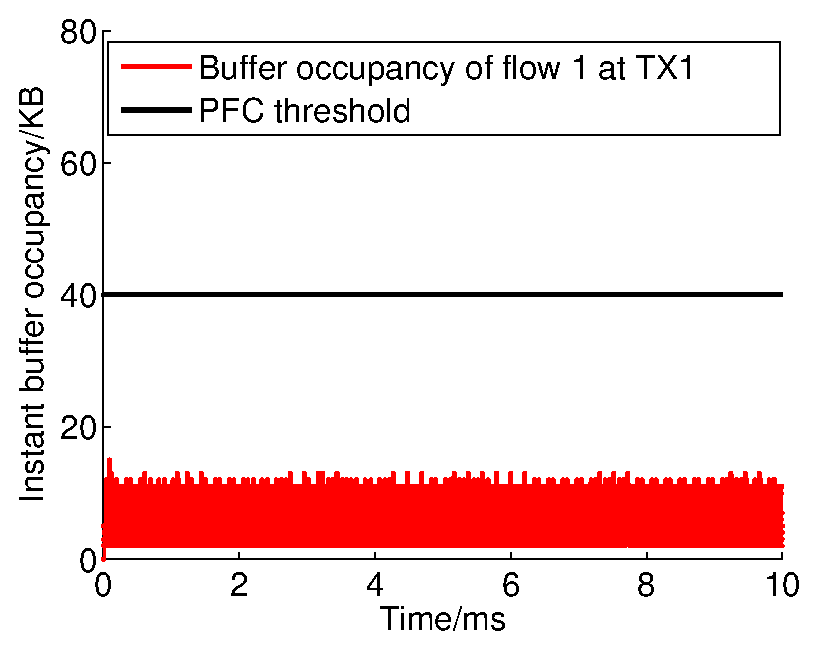
\includegraphics[width=0.23\textwidth] {figs/case1_buffer_occupancy_B.eps}
	}
	\subfigure[Buffer occupancy at switch C] {
		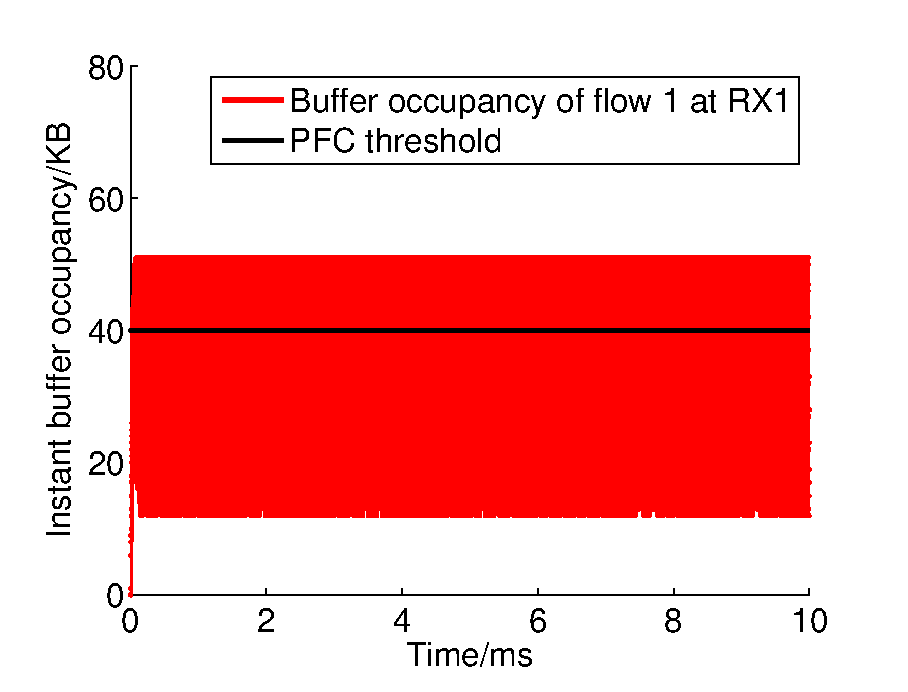
\includegraphics[width=0.23\textwidth] {figs/case1_buffer_occupancy_C.eps}
	}
	\subfigure[Buffer occupancy at switch D] {
		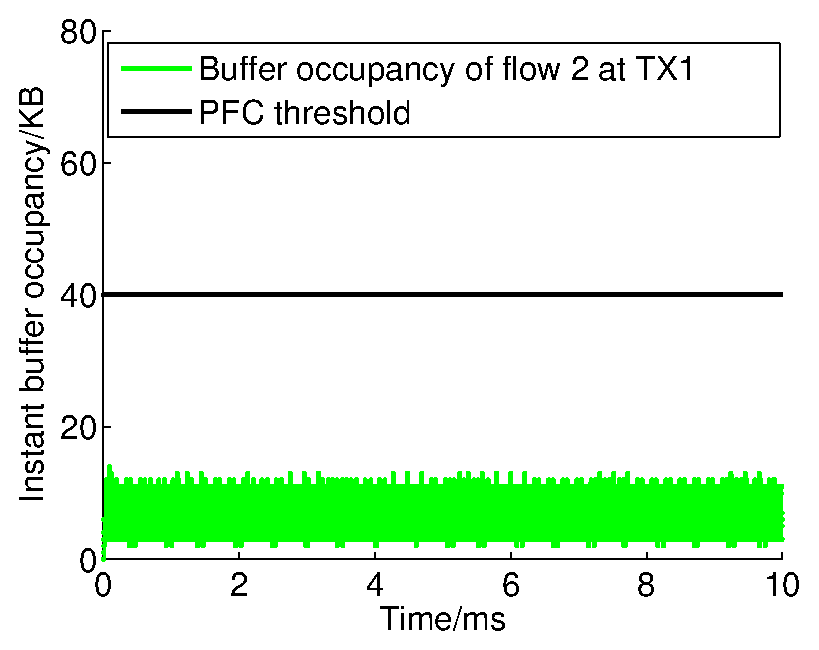
\includegraphics[width=0.23\textwidth] {figs/case1_buffer_occupancy_D.eps}
	}
	\vspace{-0.15in}
	\caption{There is no deadlock even though two flows create CBD among four switches.}
	\label{fig:case1}
	\vspace{-0.2in}
\end{figure*}


Multiple flows may create a CBD even if there is no routing loop.
Figure~\ref{fig:case1}(a) shows a simple example with four switches A, B, C and D.
Flow 1 starts at a host (not shown) attached to A, passes through B and C, and ends at a
host attached to D. Flow 2 starts at a host attached to C, passes through D and A, and
ends at a host attached to B.
Similar to the previous case, we can draw the dependency lines between switches. As shown in
Figure~\ref{fig:case1}(b), there is a CBD among the four switches, i.e.,
dependencies from RX1 of A to RX1 of B, then to RX1 of C, then to RX1 of D, and finally back to RX1 of A.


In this example, the boundary state analysis does not yield meaningful
results. Because the flows do not have any rate limiting, one can easily analyze that the
stable throughput of each flow is $B/2$. However, it is not easy to tell whether deadlock
will form. For example, one may suspect that switch A's $RX1$ will generate PFC PAUSE, and
these PAUSE frames may cascade from A to D, then to C, B and finally back to A, thus creating deadlock.
To understand such scenarios, we must analyze and simulate them at packet level.




% \textbf{Simulation setup}: To create a well-controlled experimental environment,
% we did our deadlock case study using packet-level NS-3 simulations.
%
% In our modified NS-3 simulator, we implement PFC protocol ({\em i.e.,} IEEE 802.1 Qbb protocol).
% Most modern commodity switches have a common shared buffer, while PFC works in a per ingress
% queue fashion. For each ingress queue, the switch maintains a counter to
% track its instant virtual queue length (i.e., bytes of buffered packets received by this
% ingress queue). Once the queue length of an ingress queue exceeds the pre-configured PFC
% threshold, a pause frame will be sent to the corresponding upstream device. The upstream
% device then stop sending any packet to this ingress queue unless 1) the pause frame has
% expired; 2) or it has received a resume frame from this ingress queue.
 
  \textbf{Simulation setup}: \revise{To create a well-controlled experimental environment, we simulate the scenario in Figure~\ref{fig:case1}(a) using packet-level NS-3 simulations. In our NS-3 simulator, we implement the PFC protocol ({\em i.e.,} IEEE 802.1 Qbb protocol). For each ingress queue, the switch maintains a counter to
 track the bytes of buffered packets received by this ingress queue. Once the queue length exceeds the preset PFC threshold, the corresponding incoming link will be paused.}

In our simulations, we configure static routing on all switches so that flow paths are enforced.
Both flows are UDP flows with infinite traffic demand. Link capacity of
all links is 40Gbps. All the switches have 12MB buffer. PFC threshold is statically set to 40KB for
each ingress queue. These parameters affect how fast deadlock forms (if any), but do not affect whether deadlock forms.

In Figure~\ref{fig:case1}(c), we plot the PFC pause events at four links L1, L2, L3 and L4.
If link $Li, (i=1,2,3,4)$ is paused at time $t$, we plot a point at location $(t, i)$. Pause events at
different links are plotted with different colors and of different heights. As we can observe, links
L2 and L4 are paused continuously, while the other two links L1 and L3 never get paused. In this case,
deadlock will never form as no packet will be paused permanently.

To understand the pause pattern, we sample the instantaneous buffer occupancy of
both flows at RX1 queues of A, B, C and D every 1us. In Figure~\ref{fig:case1}(d), we draw the instant
buffer occupancy of flow 2 at RX1 of A.
%Buffer occupancy of flow 1 is not drawn
%as it does not contribute to the pause of link L1 (Note that PFC works in a per ingress queue fashion).
\revise{Similarly, in Figure~\ref{fig:case1}(e), Figure~\ref{fig:case1}(f) and Figure~\ref{fig:case1}(g), we draw
the instant buffer occupancy of interested flows at RX1 queues of B, C and D, respectively. As
flow 1 and flow 2 are symmetric, we only present the analysis for Figure~\ref{fig:case1}(d) and
Figure~\ref{fig:case1}(e) to show why Link L4 is paused continuously but link L1 never gets paused.
As shown in the figures, buffer occupancy of flow 2 at RX1 of A fluctuates between 10KB
and 55KB around the PFC threshold, so link L4 will get paused intermittently. In contrast, buffer
occupancy of flow 1 at RX1 of B is well below the PFC threshold (fluctuates between 0KB and 18KB),
hence link L1 never gets paused.}

The takeaway is that, we cannot simply predict deadlock based on the existence of CBD
and flow-level stable state analysis. This is because we cannot predict
the instantaneous buffer occupancy (and whether PFC is triggered) from flow-level analysis that only
focuses on {\em average} flow throughput.

%In Figure~\ref{fig:case1}(a), packets of flow 1 and flow 2 will build up at TX1 of A as both flows are competing for the capacity of link L1. Once the buffer occupancy of flow 2 exceeds the PFC threshold, RX1 of A will generate a pause frame to TX1 of D to stop packet transmission over link L4.
%
%After link L4 is paused, buffer occupancy of flow 2 will decrease as no more packets can be received by RX1 of A. Once the buffer occupancy of flow 2 is below the PFC threshold at switch A, link L4 will be resumed. Then buffer occupancy of flow 2 will start to increase again. This is why in
%
%Since packets of flow 1 buffered in TX1 of B can get transmitted at full link speed when link L2 is not paused, TX1 queue of B can not easily build up. As we can see in Figure~\ref{fig:case1}(e), buffer occupancy of flow 1 at TX1 of B fluctuates between 0KB and 18KB, which . Hence as we can see in Figure~\ref{fig:case1}(c), link L1 is never paused by RX1 of C.

\begin{figure*}[t]
%\vspace{-0.1in}
\centering

\subfigure[Topology and flows] {
    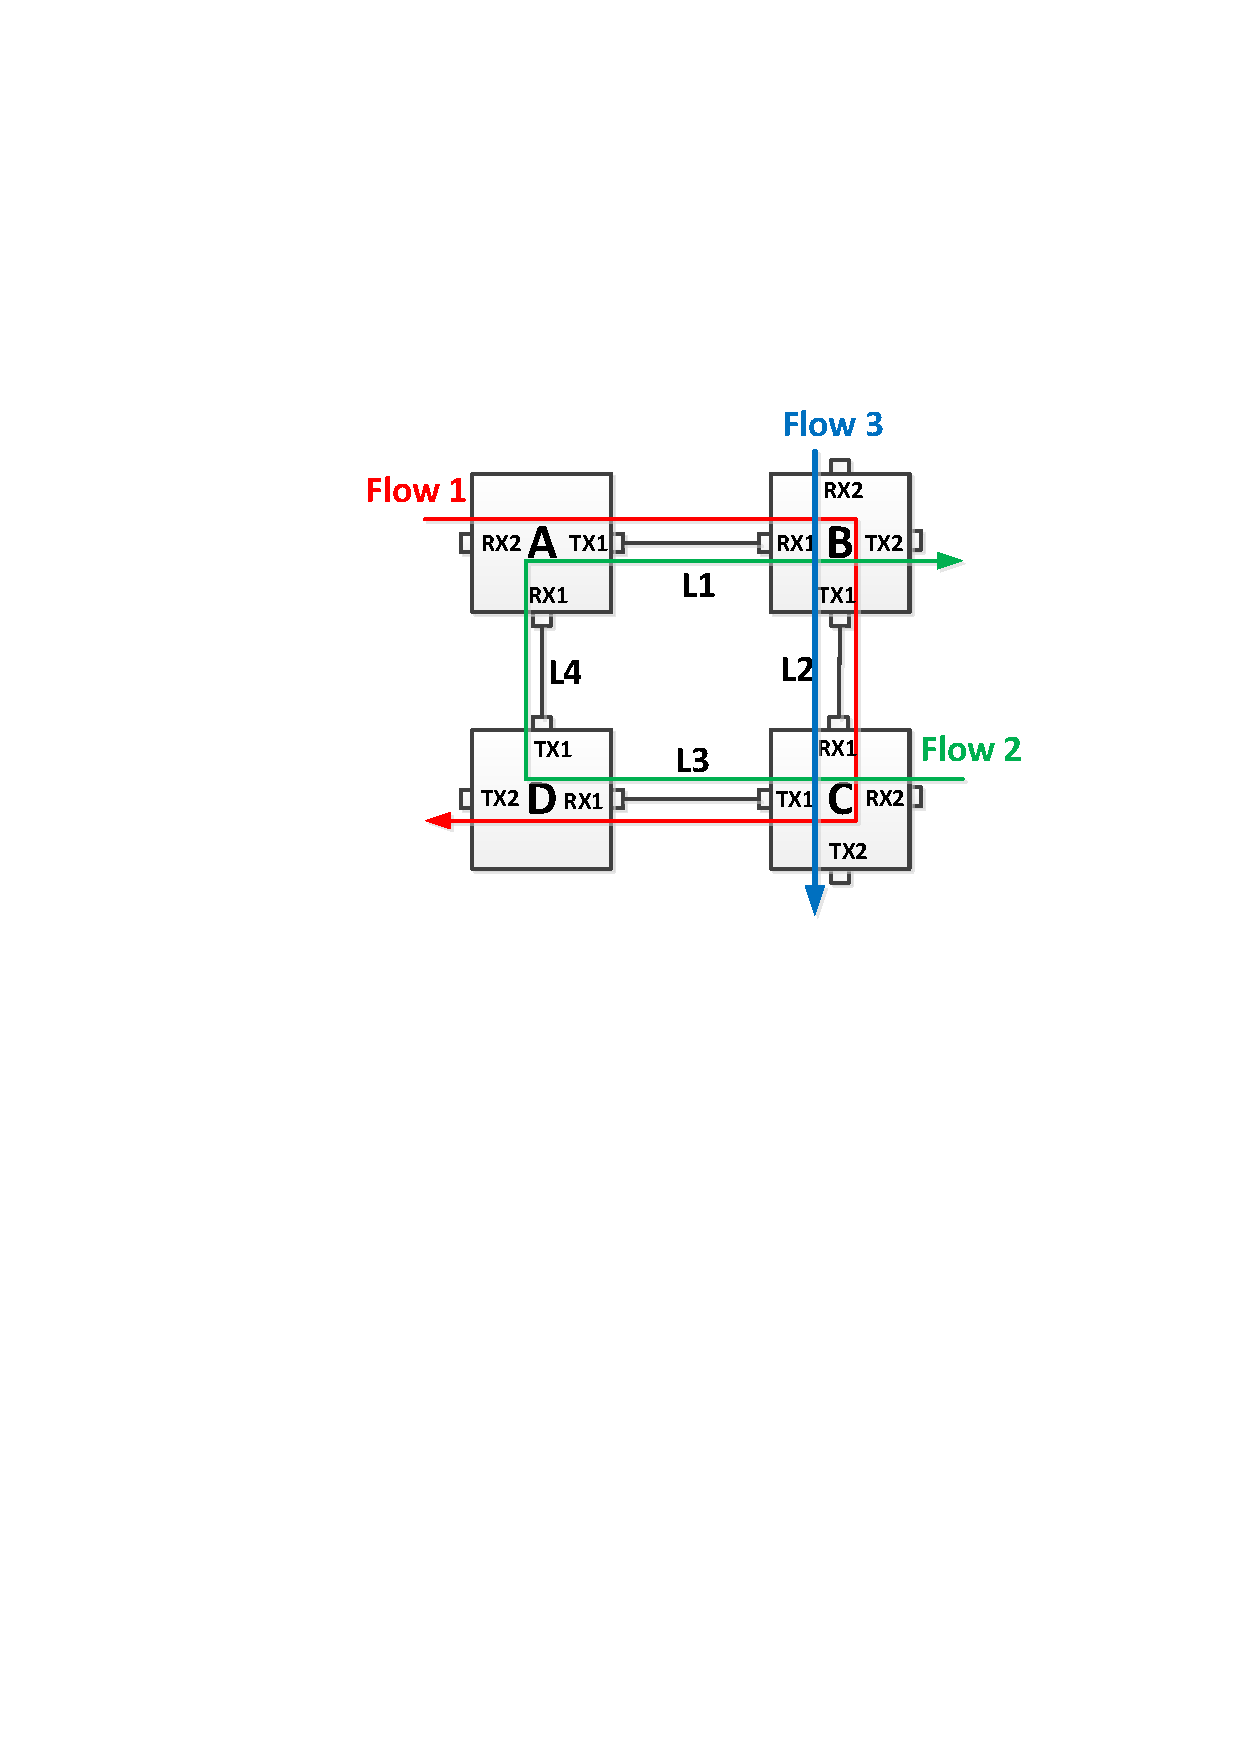
\includegraphics[width=0.25\textwidth] {figs/case2_topo}
}
\subfigure[Buffer dependency graph]{
    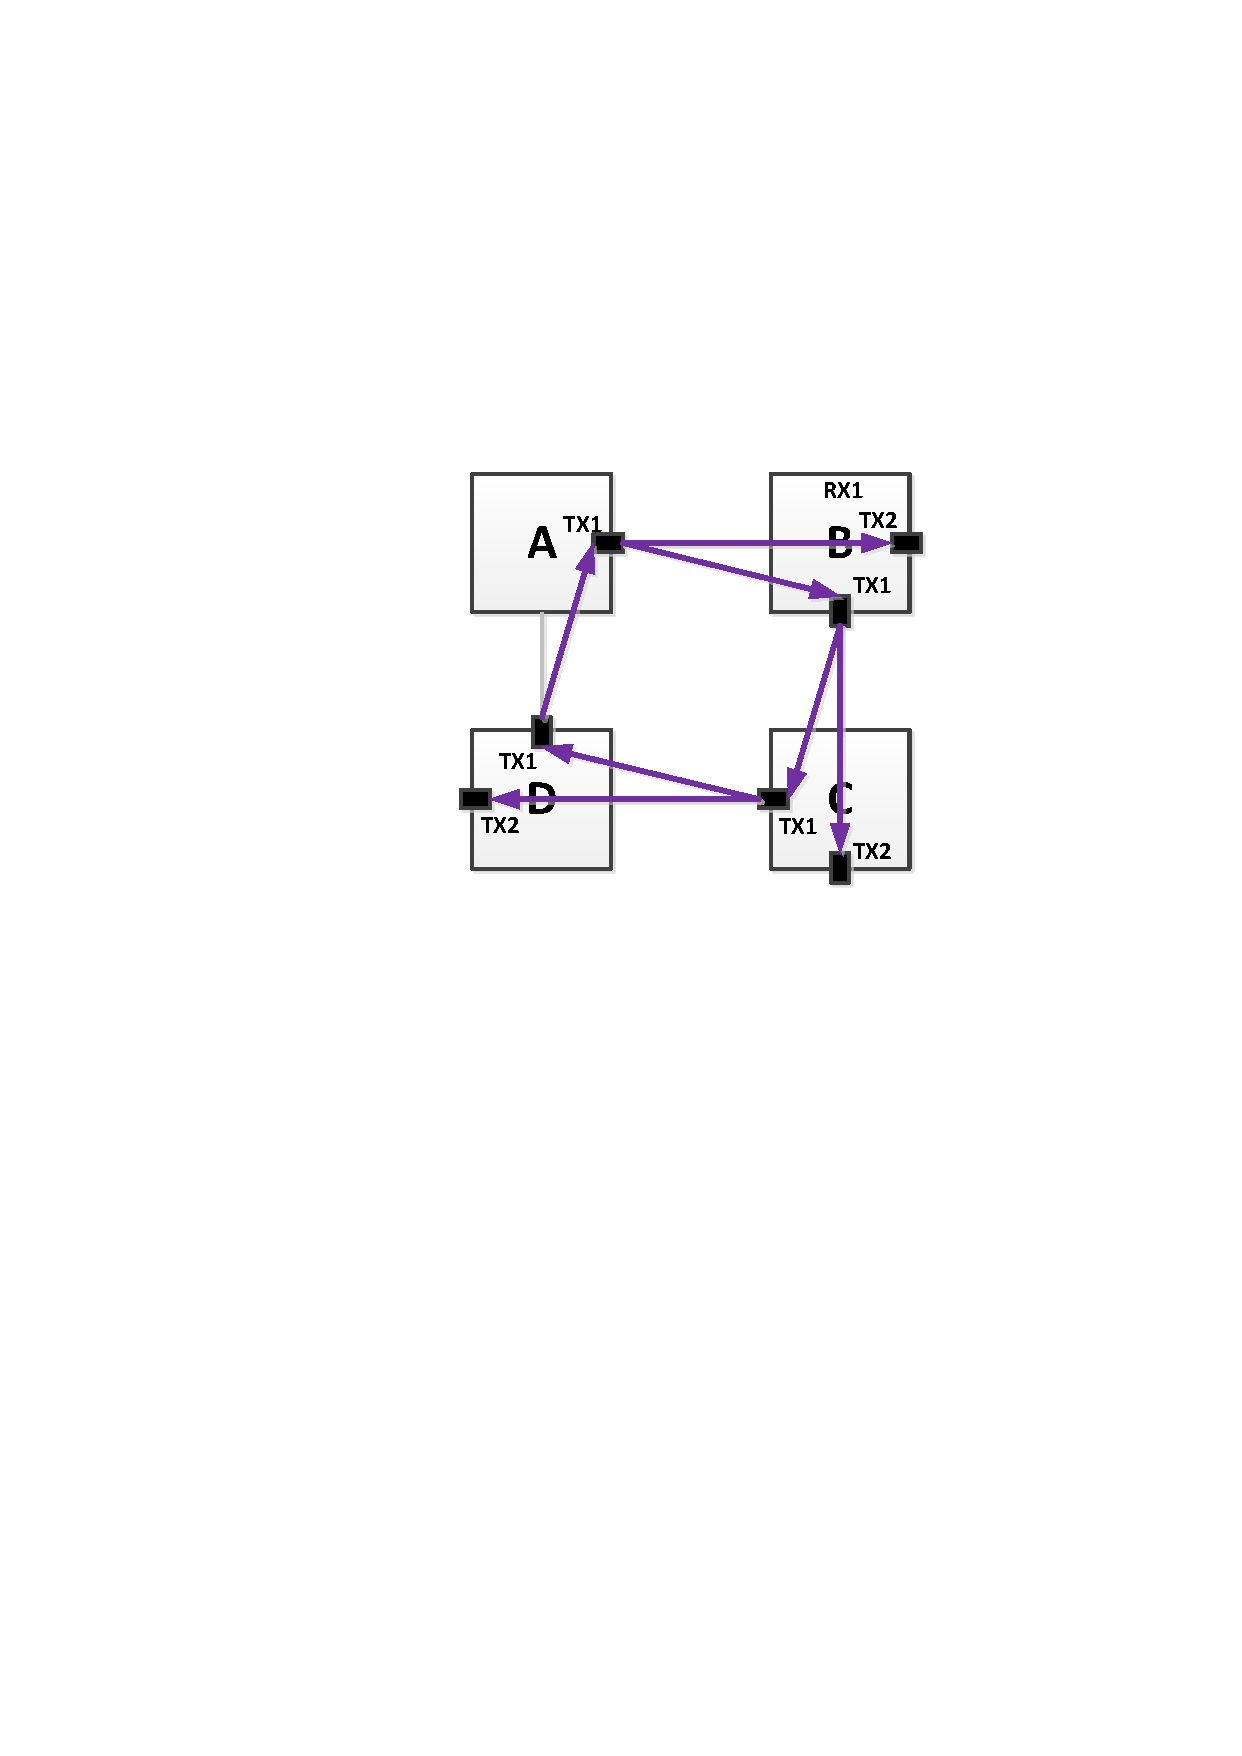
\includegraphics[width=0.2\textwidth] {figs/case2_buffer_dependency}
}
\subfigure[Pause events at four links]{
    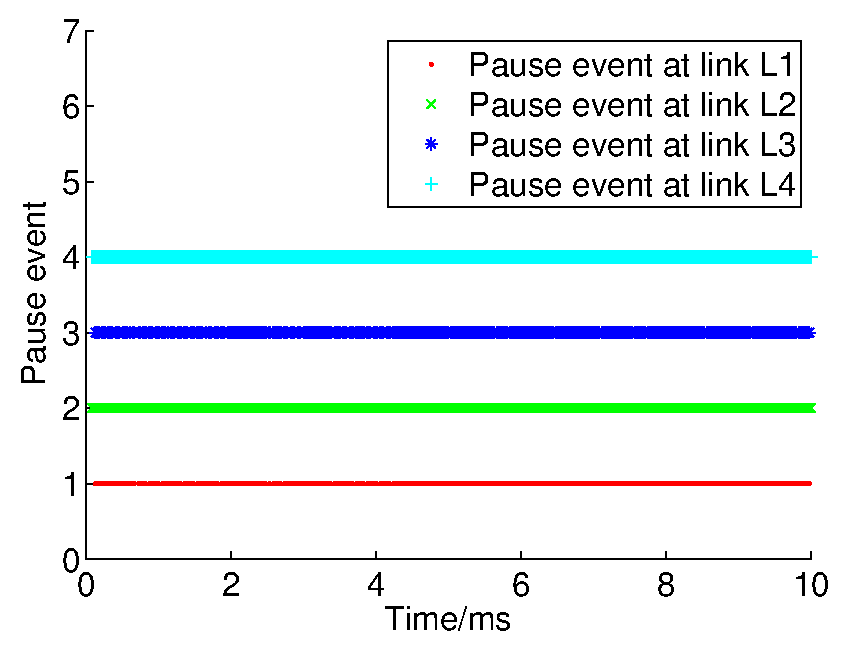
\includegraphics[width=0.22\textwidth] {figs/case2_pause.eps}
}
\vspace{-0.15in}
\caption{Slightly different traffic matrix leads to deadlock, even though
the flow-level analysis shows that the average throughput of flow 1 and flow 2 should not be affected.
}
\vspace{-0.2in}
\label{fig:case2}
\end{figure*}


\begin{figure*}[t]
%\vspace{-0.1in}
\centering

\subfigure[Topology and flows] {
    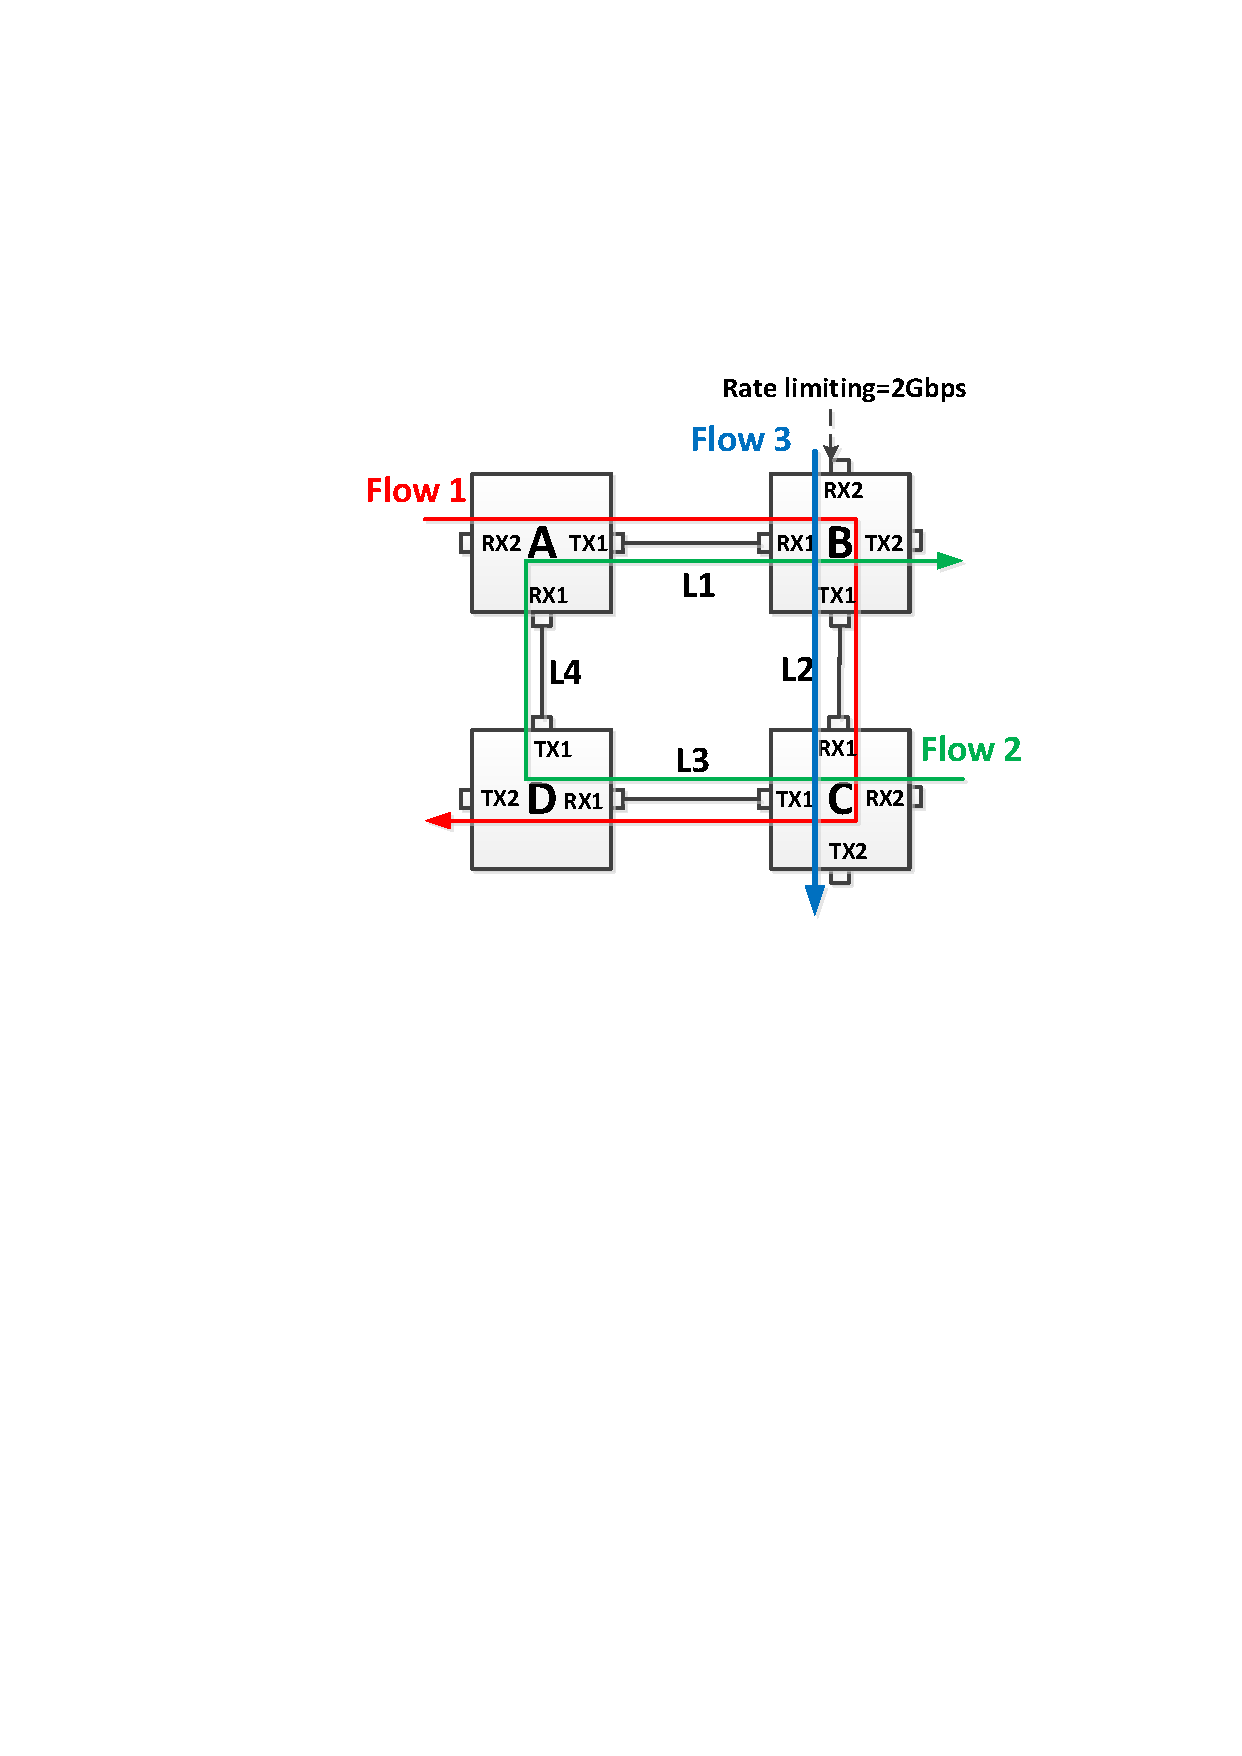
\includegraphics[width=0.22\textwidth] {figs/deadlock_case_4_topo}
}
\subfigure[Pause events at four links]{
    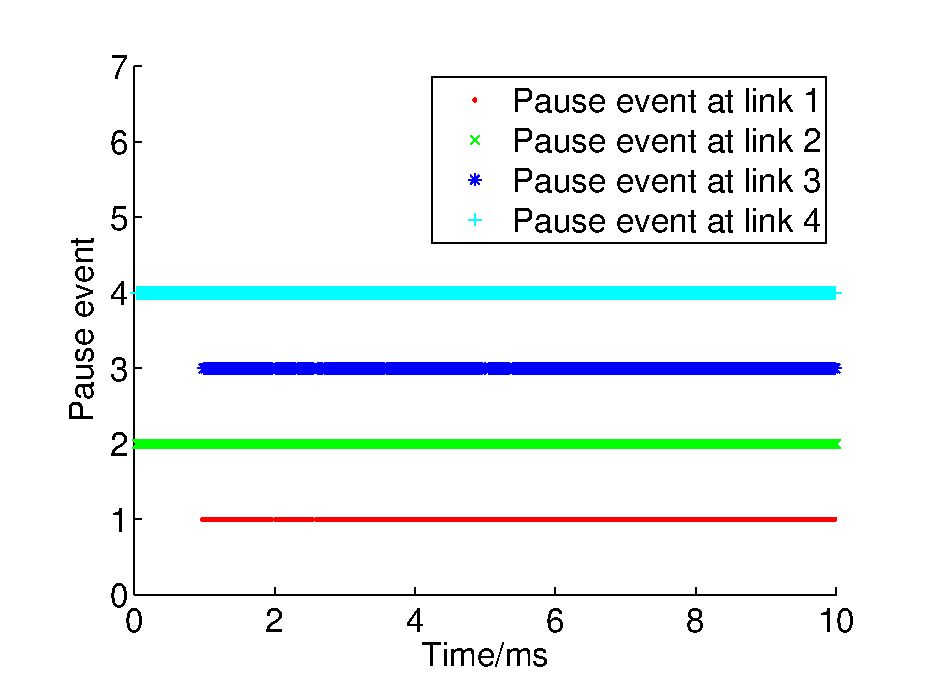
\includegraphics[width=0.22\textwidth] {figs/pause_event_limit2G.eps}
}
\subfigure[2Gbps rate limiter, no deadlock]{
    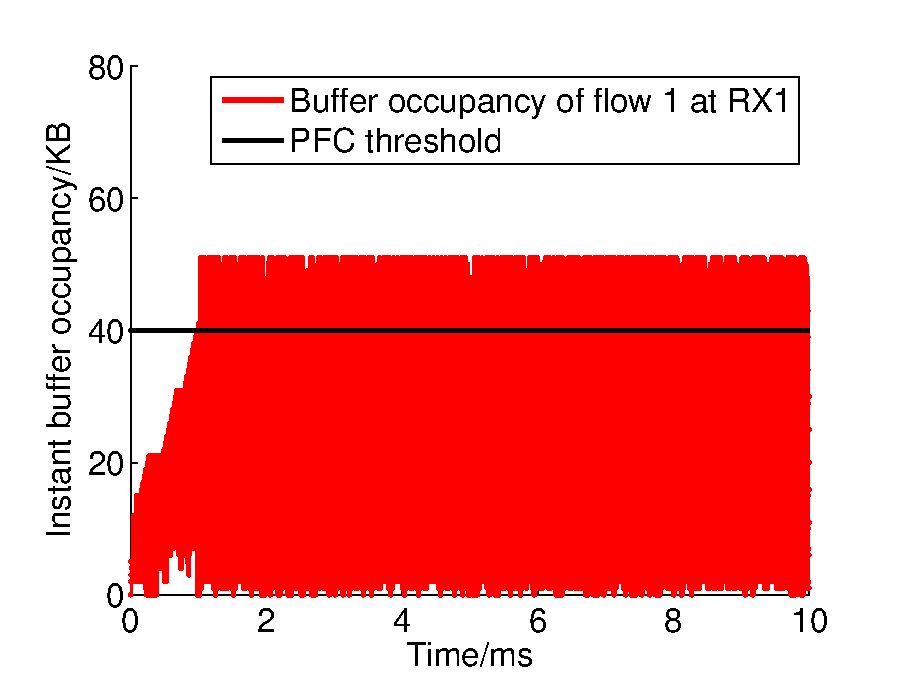
\includegraphics[width=0.22\textwidth] {figs/buffer_occupancy_B_limit2G.eps}
}
\subfigure[3Gbps rate limiter, deadlock]{
    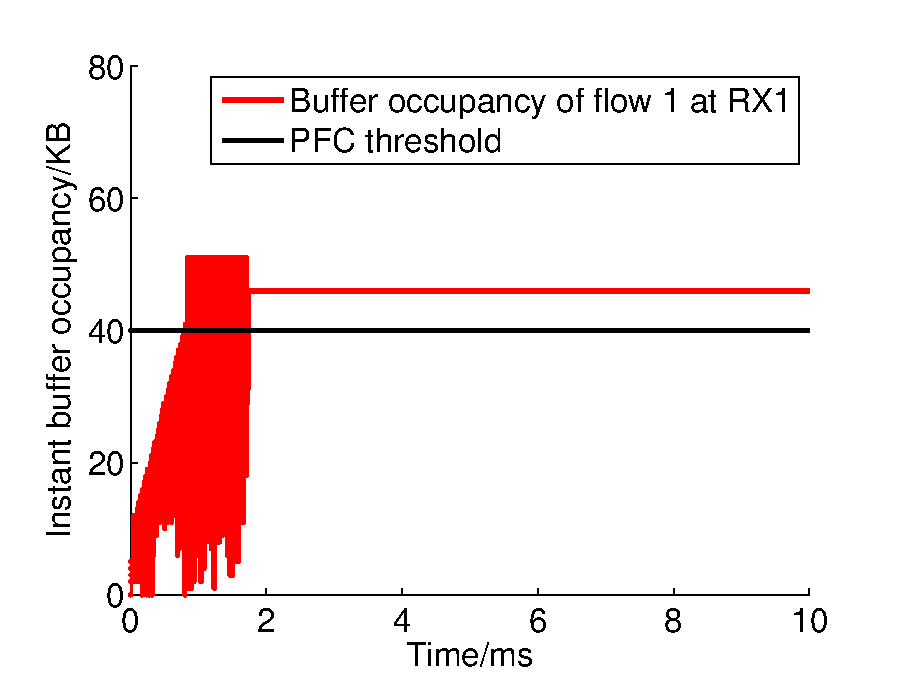
\includegraphics[width=0.22\textwidth] {figs/buffer_occupancy_B_limit3G.eps}
}
\vspace{-0.15in}
\caption{Different rate limiting determines whether the deadlock forms.}
\vspace{-0.2in}
\label{fig:case3}
\end{figure*}


\para{Slightly different traffic matrix leads to deadlock:} \revise{as shown in Figure~\ref{fig:case2}(a), based on the previous scenario, We add another flow (flow 3) which enters the network at switch B and leaves at switch C. All the three flows are UDP
flows with infinite traffic demand. Buffer dependency graph is drawn in Figure~\ref{fig:case2}(b).
Compared with previous scenario, one additional dependency from RX2 of B to RX1 of C is added, but it
is outside the CBD. The CBD itself remains unchanged.}

Pause events at four links L1, L2, L3 and L4 are plotted in Figure~\ref{fig:case2}(c). As we can see, in
this case four links are all paused. To check whether deadlock will form in this case, we stop the three
flows after a sufficient long period (1000ms). We find that pause events are continuously
generated at all the four links even after three flows stop sending new packets.
This means that a deadlock has been created among the four switches.

The bizarre thing is, if we apply the stable state flow analysis based on PFC fairness,\footnote{PFC
ensures per-hop per-port fairness. If packets from two ingress ports go to the same egress port, each ingress
port gets half of the egress bandwidth.} it is easy to see that all flows should have 20Gbps throughput.
Particular at switch D, the stable ingress and egress rate of flow 1 and flow 2 should remain the same as
the previous case (Figure~\ref{fig:case1}). However, now switch D starts to generate PFC at RX1 towards
switch C, as opposed to no PFC generated in the previous scenario.


Flow-level stable state analysis cannot capture such behavior. We can only get answers from the
packet-level analysis. Unfortunately, we have not yet found any analytic tools that can precisely
describe the PFC behaviors in these two examples. Looking at the packet traces, we only roughly know that
after adding flow 3, flow 1 has to share the bandwidth of link L2 with flow 3 and this may cause
different PFC patterns on link L1 without affecting the average throughput of flow 1 and flow 2.
\revise{But this change in pattern makes PFC cascade towards L4 and finally L3.}

%packets of flow 1 buffered in TX1 of B can no longer get transmitted at full link
%speed due to the contention with packets of flow 3. Packets of flow 1 will then build up at TX1 of B.
%Once the packets of flow 1 buffered at TX1 of B exceed the PFC threshold, RX1 of B will send a pause
%frame to TX1 of A to pause Link L1. The pause on link L1 will help packets to build up at TX1 of A,
%and has a cascade effect on link L4. Due to the pause at link L1, link L4 will get paused more frequently.
%Then packets of flow 2 are easier to build up at TX1 of D. Once the PFC threshold is triggered at D,
%link L3 also get paused. So in case 2, pause events can occur at all the four links.

Once all the four links are paused simultaneously, there is a chance that no link can get resumed.
For example, it is possible that when simultaneous pause happens, at switch A and switch B, the
first packet buffered in the head is a packet of flow 1, and meanwhile, at switch C and switch
D, the first packet buffered in the head is a packet of flow 2. \revise{Once this condition is met, PFC deadlock occurs.} 

%In this case, all the queues are waiting for its downstream neighbors to release some
%buffer to break the standstill condition.

\para{Summary:}
In the above multi-flow scenarios, CBD can be created without
a routing loop. However, it is again not a sufficient condition for deadlock. The analysis of sufficient
condition is complicated. Stable flow state analysis does not apply.
A slightly different matrix that does not significantly affect stable flow state may lead
to very different packet-level behavior, thus different deadlock results.
Though packet-level simulations help us understand these scenarios, we so far do not find
any analytic tools that are at packet-level and work for above examples.

\secspace
\subsection{Case 3: Rate Limiting Mitigates Deadlock}
\secspace

In the last deadlock example (Figure~\ref{fig:case2}), if we additionally limit the rate of flow 3, deadlock
may be avoided.  As shown in Figure~\ref{fig:case3}(a), we add a rate limiter to switch B's
ingress port RX2. While the buffer dependency graph remains the same as Figure~\ref{fig:case2}(b),
slower flow 3 means that the congestion on switch B is reduced, PFC is less
frequent and deadlock may be avoided. The question is, what is the maximum rate that can
avoids deadlock?

Again, using flow-level stable state analysis, we cannot get the answer. We use packet-level simulator
to test different rate limiting values. We find that when the rate of flow 3 is no more than 2Gbps,
there is no deadlock even though all links have frequent PAUSE (Figure~\ref{fig:case3}(b)).
Note that, after zoom in Figure~\ref{fig:case3}(b), we can see that four links are {\em never} paused
simultaneously at packet level. Why is 2Gbps different from higher rate, like 3Gbps?

We plot the buffer occupancy of RX1 at switch B, and compare when we limit the rate of RX2 to 2Gbps
(Figure~\ref{fig:case3}(c)) and 3Gbps (Figure~\ref{fig:case3}(d)). Interestingly, the buffer occupancy
always fluctuates between 0 and a little above PFC threshold\footnote{It takes some time for PFC PAUSE
to arrive the other side and become effective after PFC threshold is reached.
The switch buffers additional packets due to this delay.} with 2Gbps rate limiter. While with 3Gbps rate
limiter, after some fluctuation the buffer goes into deadlock, even though the peak buffer usage is the same
as 2Gbps case. Unfortunately, we cannot find any existing analysis tools that explain
what we have observed.

In short, while rate limiting mitigates deadlock, packet-level analysis is required for understanding
the actual threshold. We are currently working on analysis tools, {\em e.g.,} a fluid model that
can describe PFC behavior, and will report it in future work.



%This rate limiter on switch C pushes back flow 3 by generating PFC PAUSE
%at port RX2 towards switch B (and switch B further pushes back the host).
%Note that the PAUSE of flow 3 at L2 can cause Head-of-Line (HoL) blocking for flow 1 packets on
%the same link. if this HoL blocking is serious enough, the flow 1 packets can build up a queue
%at at switch B and the PFC may cascade further .As a result, we
%observe frequent PFC PAUSE on all L1, L2, L3 and L4, as shown in Figure~\ref{fig:case3}(b).




\if 0
\textbf{Case 3:} In this case, we will show that even if all the four links are paused simultaneously,
it is not guaranteed that a deadlock will be created. As shown in Figure~\ref{fig:case3}(a), in addition
to case 1, we add another two flows (flow 3 and flow 4). Flow 3 starts at a host attached to A, passes
through A and B, and ends at a host attached to B. Flow 4 is a symmetric flow of flow 3 that runs over
C and D. All the four flows are UDP flows with infinite traffic demand. Two rate limiters are added at
TX3 queues of B and D to ensure that rates of flow 3 and flow 4 will not exceed $1/4$ of the link
capacity. Buffer dependency graph of case 3 is drawn in Figure~\ref{fig:case3}(b). Compared with case 1,
two additional buffer dependencies from TX1 queues to TX3 queues are added.

Pause events at four links L1, L2, L3 and L4 are plotted In Figure~\ref{fig:case3}(c).  As we can see
from the figure, all the four links are paused continuously. However, we find that once we stop the
flows, all the links get resumed and buffer occupancy of four switches soon becomes zero. This
indicates that deadlock cannot be created in case 3.

To find out why there is no deadlock in case 3, we draw the instant buffer occupancy of 3 flows at
switches A and B in Figure~\ref{fig:case3}(d), Figure~\ref{fig:case3}(e) and Figure~\ref{fig:case3}(f).
Here we omit the buffer occupancy condition of switches C and D as the topology and the flows are symmetric.

As shown in Figure~\ref{fig:case3}(d), at TX1 of A, the buffer occupancy of flow 2 exceeds the PFC
threshold, so link L4 will get paused. To understand why link L1 is also paused, we need to consider
the buffer occupancy of flow 1 and flow 3 at switch B. The reason is that packets received by RX1 of
B are possible to be queued at both TX1 and TX3 (note that there is a rate limiter on TX3). As long
as the sum of the buffer occupancies of both TX queues exceeds the PFC threshold, link L1 will get paused.
As we can see in Figure~\ref{fig:case3}(e) and Figure~\ref{fig:case3}(f), although individually buffer
occupancy of either TX1 or TX3 is less than the PFC threshold, their sum is larger than the PFC
threshold. Hence link L1 is paused.

As both TX1 and TX3 contribute to the pause on link L1, to create a deadlock, we need to ensure that
packets buffered at both TX queues cannot get resumed. However, packets buffered at TX3 can always get
transmitted within a finite time as it is not involved in any CBD. This explains
why when we stop the flows, all the four links can be resumed from the pauses.
\fi

%\textbf{Observation 3:} even if all the links in a cycle are paused simultaneously, it is not
%sufficient to create a permanent deadlock.

\para{Summary:} From all the examples in this section, we summarize that CBD is
 a loose condition for deadlock. The traffic demand matrix, TTL and flow rates all affect the deadlock
 formation. While we cannot obtain the tightest condition ({\em i.e., necessary and sufficient condition}),
we know that a tighter condition should include those factors, and that these factors can be utilized
for deadlock mitigation. In Section~\ref{sec:mitigation}, we discuss potential deadlock mitigations in
addition to avoiding CBD.

%\subsection{Deadlock problem in RDMA DCNs}\label{subsec:deadlock_problem}
%
%Once a loop occurs in a network, packets of some flows will be caught in the loop and traverse the same links multiple times until they are dropped due to Time-to-Live (TTL) expiration. Apart from causing packet drops, loops will also waste some link bandwidth as well as increase the end-to-end delay for the flows traversing some link(s) in the loop (but not caught by the loop).
%
%\begin{figure}[t]
%\centering
%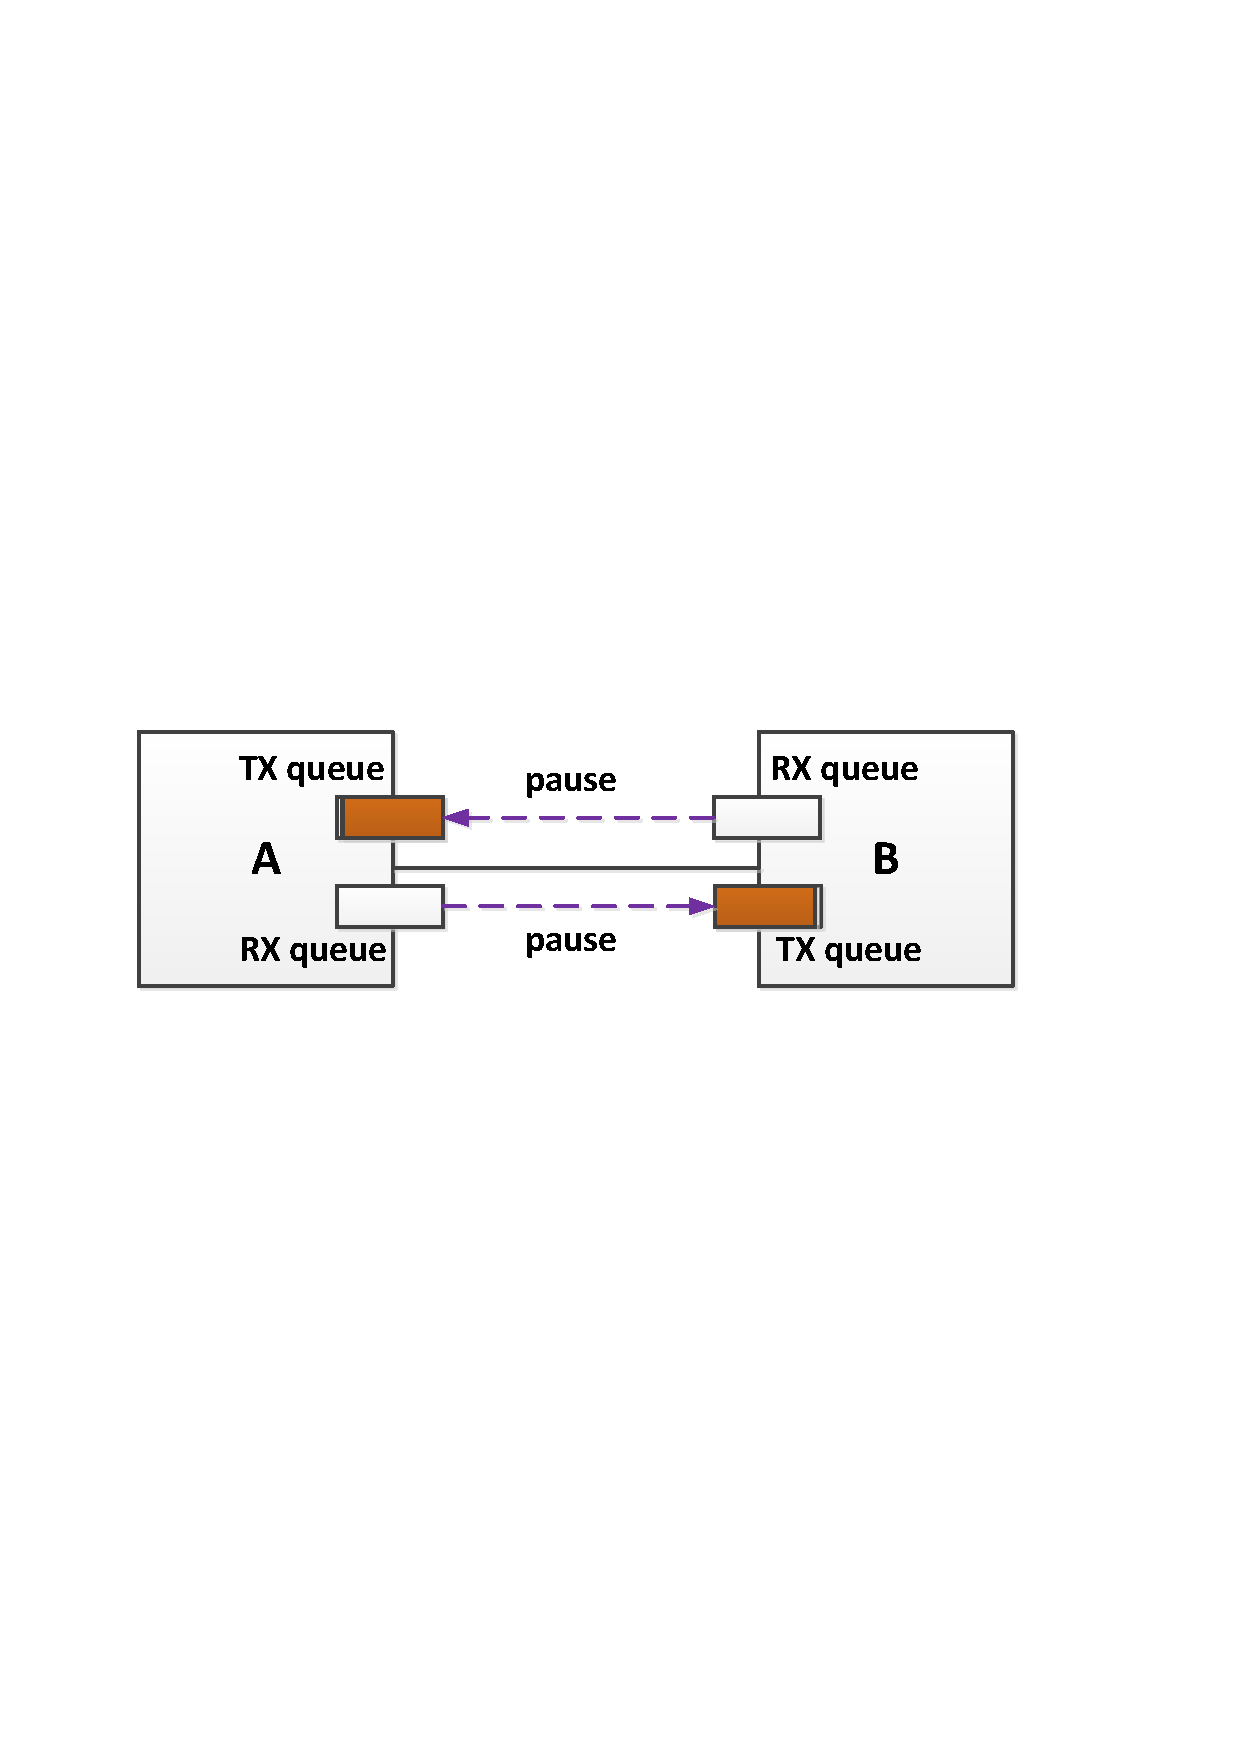
\includegraphics[width=0.45\textwidth,center]{figs/deadlock_example.pdf}
%\caption[Optional caption for list of figures]{An example of loop induced deadlock: there is a loop between switch A and switch B. Both TX queues (egress queues) are paused by PFC as no buffer are available at both switches to accommodate more packets.}
%\label{fig:loop_deadlock}
%\end{figure}
%
%In a lossy network, the impact of a loop is not fatal and can be completely eliminated as long as the loop is removed from the network. In contrast, in a lossless network, if packets enter a loop faster than they get dropped in the loop due to TTL expiration, packets will occupy the buffer of all the switches in the loop, and then a deadlock is created. When a deadlock occurs, each switch in the loop is paused by its downstream switch, and at the same time pauses its upstream switch due to the lack of available buffer to accept more packets. Once such a circular buffer dependency is created, the deadlock condition will hold persistently even after the loop is eliminated.
%
% Under deadlock condition, no packets can move along the links in the loop, and more and more devices outside the loop will be paused due to the cascade effect of PFC. If a deadlock is created in the core of the network, it is very likely to bring the whole data center into a deadlock state.
%
%A simple deadlock example is shown in Figure~\ref{fig:loop_deadlock}. In this example, there is a routing loop between switch A and switch B. Packets enter this loop at a sufficient large rate and soon occupy all the available buffer of both switches. Then Both TX queues (egress queues) will be paused by PFC PAUSE frames and a deadlock is created. As we can see, this deadlock cannot be resolved by eliminating the routing loop as packets are already queued in the TX queues and can never reach the next-hop switch to escape from the loop.
%
%\subsection{Sufficient condition for deadlock creation}\label{subsec:deadlock_condition}
%
%In this part, we analyze the sufficient condition to create a deadlock when there is a loop in the network.
%
%At first, we consider the maximum packet drain rate in a loop regarding TTL expiration. Let $n$ the number of switches in a loop, $B$ be the link bandwidth and $k_{TTL}$ be the TTL value of packets before they enter the loop. Each time a packet traverses one switch, its TTL value will be reduced by 1.
%
%The maximum packet drain rate is achieved when no switch is paused by PFC PAUSE frame and each switch is sending packets to its next-hop in the loop at the rate of $B$. So the maximum packet drain rate $r^{max}_d$ is equal to $nB/k_{TTL}$. here $nB$ can be viewed as the maximum packet ``flowing" rate in the loop, while $1/k_{TTL}$ captures the information that a packet will be dropped after it has traversed $k_{TTL}$ hops of switches in the loop.
%
%Let $r_{in}$ be the injection rate of packets into the loop. One sufficient condition to create a deadlock in a lossless network is that: there is a loop
%in the network, and condition $r_{in} > r^{max}_d$ holds for a sufficient long period until a circular buffer dependency is created in the loop.
%
%\begin{figure}[t]
%\centering
%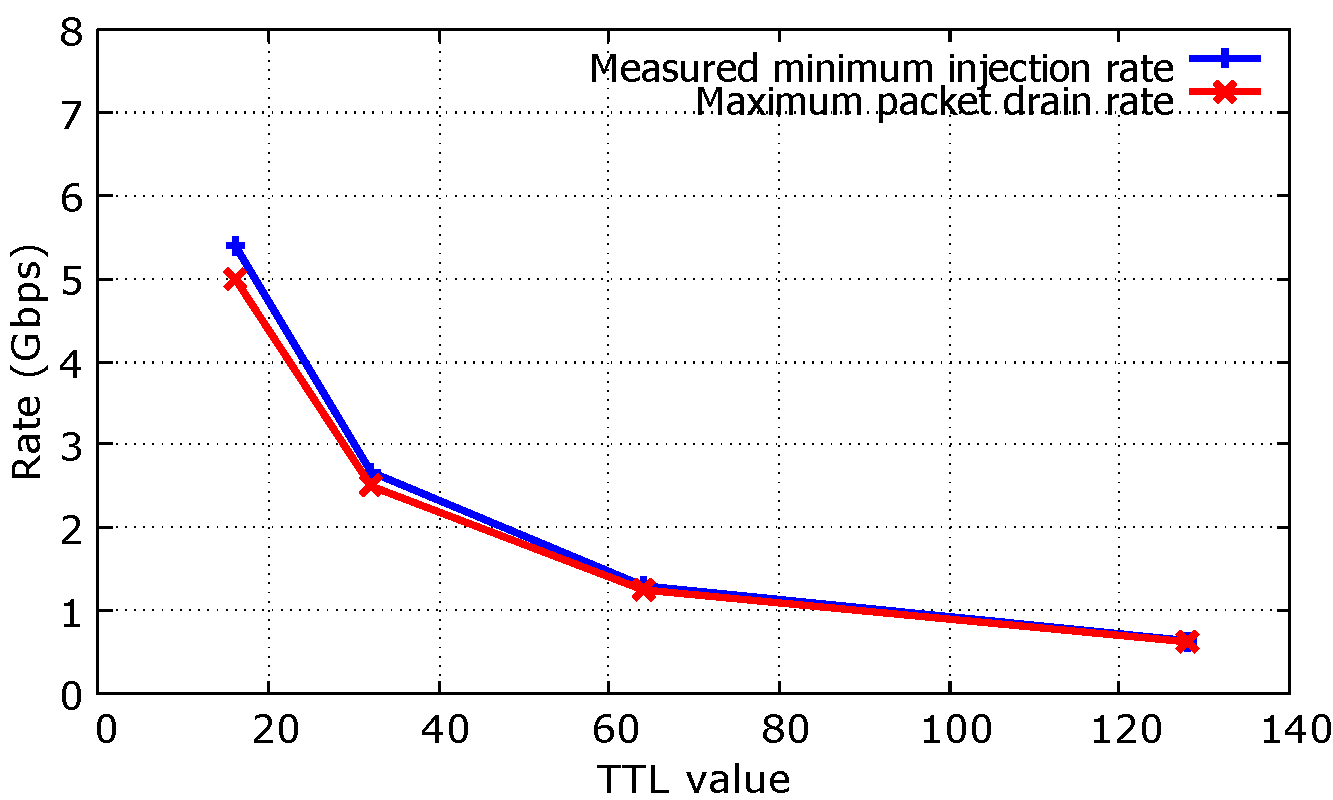
\includegraphics[width=0.5\textwidth,center]{figs/r_and_rdrain.pdf}
%\caption[Optional caption for list of figures]{Measurement of the minimum injection rate to create a deadlock. Both switches in the loop are Arista 7050QX32.}
%\label{fig:mrate_measurement}
%\end{figure}
%
%To verify our analysis above, we manually configure a loop between two 40Gbps switches, and measure the minimum packet injection rate that can create a deadlock. The result is shown in Figure~\ref{fig:mrate_measurement}. As we can see, the measured minimum packet injection rate is just slightly larger than the maximum packet drain rate which is computed according to $nB/k_{TTL}$. This observation holds when TTL is set to different values.
%
%Another observation from the figure is that, setting smaller TTL can help to prevent deadlock but its benefit is limited. As shown in the figure, when TTL is set to 16 which is already a very small value, the minimum injection rate is only about 6Gbps.
%
%\subsection{Analysis of the time to create a deadlock}\label{subsec:deadlock_condition}
%
%In this part, we analyze and measure the time to create a deadlock when the sufficient condition for deadlock creation is already met. Deadlock creation time is related to three factors: \textbf{packet injection rate $r_{in}$}, \textbf{packet drain rate $r_{d}$} and \textbf{PFC threshold $t_{PFC}$}.
%
%$t_{PFC}$ determines the minimum bytes of packets needed to be ``trapped" in the loop to create a deadlock, while $r_{in} - r_{d}$ can be viewed as the packet increase rate.
%
%%Packet injection rate is determined by the instant traffic demand of applications running in the data center. A larger injection rate requires less time to create a deadlock.
%%
%%As discussed above, the maximum packet drain rate will be a fixed value once $n$, $B$ and $k_{TTL}$ is determined. We find that packet drain rate will decrease significantly after packets are queued in the loop because it will take a packet much longer time to get dropped in the loop when there is queuing delay.
%
%Most modern commodity switches use a dynamic $\alpha$ algorithm to determine the value of PFC threshold: Let $\alpha$ be a parameter with the range from 0 to 1, $m$ be the total switch buffer size and $m^\prime$ be the amount of buffer currently occupied. For a given $\alpha$, the value of $t_{PFC}$ is dynamically computed according to the following equation $ t_{PFC} = \alpha(m - m^\prime)$. During runtime, once the queue length of an ingress queue exceeds the instant $t_{PFC}$, a PAUSE frame will be sent to its upstream device. Note that a PAUSE frame will take some time to arrive an upstream device and take effect. To avoid packet loss due to this delay, some buffer headroom must be reserved for each ingress queue, and hence the value of $m$ in the equation is usually slightly smaller than the total switch buffer size.
%
%%
%
%
% %Most modern commodity switches share memory buffer among all ports. In order to better utilize the available shared buffer in a timely fashion, instead of setting a fixed PFC threshold,
%%A PAUSE frame will take some time to arrive an upstream device and take effect. To avoid packet loss due to this propagation delay, we must reserve enough
%%buffer headroom for each ingress queue to accommodate packets a switch may receive before a PAUSE frame finally takes effect. Let $\Delta m$ be the total amount of reserved buffer headroom. The $m$ in the above equation should be modified to be $m - \Delta m$.
%%Switches and NICs will track the value of $m^\prime$ and update the value of $t_{PFC}$ during runtime.
%
%%A smaller $\alpha$ value can lead to a shorter creation time of deadlock.  This is because a smaller $\alpha$ value means a smaller PFC threshold, while a smaller PFC threshold requires less packets to trigger a switch queue to send PAUSE frames to stop its upstream neighbors.
%
%In the next, we measure the time to create a deadlock when setting different $\alpha$ and TTL values.
%
%
%\begin{figure}[t]
%\centering
%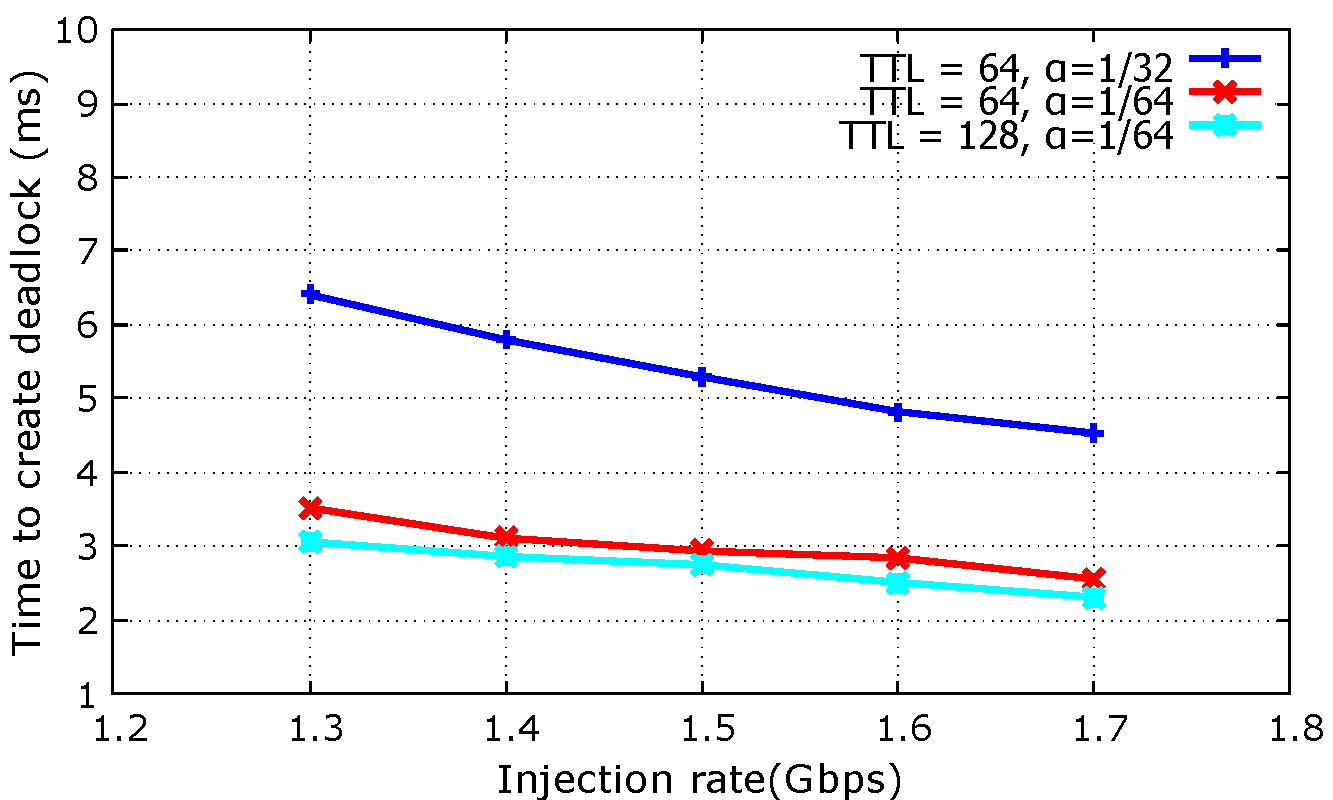
\includegraphics[width=0.5\textwidth,center]{figs/r_dltime.pdf}
%\caption[Optional caption for list of figures]{Measurement of the time to create a deadlock under different settings (deadlock will not occur when the injection rate is less than 1.3Gbps).}
%\label{fig:dltime_measurement}
%\end{figure}
%
%\parab{Measurement of the time to create a deadlock:} We manually configure a loop between two Arista 7050QX32 switches which have 32 full duplex 40Gbps ports and 12MB shared buffer. In Figure~\ref{fig:dltime_measurement}, we set $\alpha$ and $TTL$ to different values and measure the time to create a deadlock under different injection rates.
%
%We can make four observations from the results in Figure~\ref{fig:dltime_measurement}: 1) It takes only a few milliseconds to create a deadlock even when the injection rate is less than 2Gbps. This indicates that it is easy for a deadlock to occur even when only a transilient loop exists in the network. In addition, we cannot rely on any loop detection and recovery solutions to prevent the occurance of deadlocks as they are too slow to resolve the loop within a few milliseconds. 2) As the injection rate increases, the time to create a deadlock decreases accordingly. 3) Given a fixed injection rate, a smaller $\alpha$ value requires less time to create a deadlock. 4) Given a fixed injection rate, a smaller TTL value requires more time to create a deadlock. This is because a smaller TTL value will make the packets get dropped faster in the loop, and thus more packets are needed to be injected into the loop to trigger switch to pause each other.
%
%We repeated this experiment using many other combinations of TTL and $\alpha$ values and different number of switches. We found that all the results comply with what have been shown in Figure~\ref{fig:dltime_measurement}.
%
%The takeaway of this experiment is that: once there is a loop in the network, deadlock is easy to occur and very hard to prevent (a deadlock can be created within a few milliseconds). In addition to a fast loop detection mechanism, we need an effective solution to detect and resolve deadlocks caused by all kinds of loops.

%\parab{Estimation of the time to create a deadlock:}

%\parab{Sufficient condition for deadlock creation:} \todo{(detailed content to be added later.)}
%
%   1. Analysis of the maximum packet drain rate caused by TTL expiration: $r^{max}_d = nB/k_ttl$.
%
%   2. Using testbed experiments to demonstrate that $r > r^{max}_d$ is a sufficient condition for deadlock creation.
%
%\parab{Creation time of deadlock:} \todo{(detailed content to be added later.)}
%
%   1. Analysis of the upper bound and lower-bound of the creation time of deadlock.
%
%   2. a) Using testbed experiments to demonstrate that lower-bound value is already a tight estimation when $r << B$; b) Analysis of the impact of PFC PAUSE frames on $r$ and $r^{max}_d$.
%
%\subsection{Analysis of device bug induced deadlock}\label{subsec:analysis_loop_deadlock}
%\todo{to be added.}
